\subsection{SP-10 (KAB)}
Symetrické šifry blokové a proudové, základní parametry, operační módy blokových šifer, jejich základní popis a slabiny.

Symetrické šifry používají pro operaci šifrování a dešifrování stejný klíč (případně snadno převeditelný).

\subsubsection*{Proudové šifry}
\begin{itemize}
	\item proudová šifra zpracovává každý znak zvlášť
	\item na každý znak je použita jiná šifrovací transformace $E_{h_i}$, která je posunem v abecedě o $h_i$ znaků
	\item posloupnosti $h_1, h_2, ...$ se říká key-stream, a je vygenerována z klíče
	\item synchronní šifry: key-stream je závislý pouze na klíči (vypadne znak --- zbytek textu už nerozšifrujeme)
	\item asynchronní šifry: key-stream je závislý jak na klíči, tak na předchozích zpracovaných datech (takže na OT a/nebo ŠT) (vypadne znak --- po $n$ znacích jsme schopni zase dešifrovat správně)
	
	\item příklad šifer: RC4, Salsa20, ChaCha, A5/1
\end{itemize}


\subsubsection*{Blokové šifry}
\begin{itemize}
	\item šifrují $t$ znaků najednou (bloky délky $t$)
	\item všechny bloky jsou šifrovány tou samou transformací
	\item DES, 3DES --- 64b blok, DES 56b klíč, 3DES 112b/168b klíč
	\item AES --- 128b blok, 128b/192b/256b klíč
	\item šifra Feistelova typu --- postupná aplikace relativně jednoduchých operací, vytvoří poměrně složitý algoritmus
	\item iterativní bloková šifra --- základem je jednoduchá funkce provádějící šifrování jednoho bloku, která je několikrát zopakována na tom samém bloku --- jedna iterace se jmenuje 1 runda
	\item DES --- 16 rund, z 56b klíče se expandují rundovní klíče, v praxi nevýhoda krátkého klíče
	\item 3DES --- kombinace 3 operací DES za sebou, s použitím 2 nebo 3 různých DES klíčů ($E_{K_1}$, $D_{K_2}$, $E_{K_{1/3}}$)
	\item AES --- 10/12/14 rund v závislosti na délce klíče --- není Feistelova typu, nemá slabé klíče, odolná proti různým útokům
	\begin{itemize}
		\item stav = 1 blok (16B) v matici 4x4
		\item Expanze klíče --- z klíče se odvodí rundovní klíče
		\item AddRoundKey (xor rundovního klíče se stavem)
		\item Iterace/runda: SubBytes (náhrada bytů dle tabulky), ShiftRows (posunuti bytů cyklicky v řádcích), MixColumns (vynásobení matice maticí), AddRoundKey
		\item v poslední rundě je vynechána MixColumns
	\end{itemize}
	
\end{itemize}

\subsubsection*{Operační módy}
\begin{itemize}
	\item operační módy blokových šifer nám mohou zlepšit vlastnosti blokových šifer
	\item ECB (Electronic Codebook)
	\begin{itemize}
		\item bloky jsou šifrovány i dešifrovány nezávisle na sobě
		\item stejný blok OT má stejný obraz v ŠT
		\item lze zasahovat do dat --- odebírat bloky a přehazovat
		\item 1 bit chyby v ŠT poškodí celý blok OT
	\end{itemize}
	\item CBC (Cipher Block Chaining)
	\begin{itemize}
		\item je potřeba IV
		\item každý blok OT se nejprve sečte (xor) s předchozím blokem ŠT (první IV) a následně zašifruje
		\item 1 bit chyby v ŠT poškodí celý aktuální blok OT a 1 bit z následujícího
	\end{itemize}
	\item CFB (Cipher Feedback)
	\begin{itemize}
		\item je potřeba IV
		\item dělá z blokové šifry proudovou (asynchronní/samosynchronní)
		\item každý blok OT se sečte (xor) s přechozím blokem ŠT, který byl nejprve zašifrován klíčem (IV pro první blok)
		\item 1 bit chyby v ŠT poškodí celý příští blok OT a 1 bit z aktuálního
	\end{itemize}
	\item OFB (Output Feedback)
	\begin{itemize}
		\item je potřeba IV
		\item dělá z blokové šifry proudovou (synchronní)
		\item každý blok OT se sečte (xor) s aktuálním heslem z key-streamu, key-stream je nezávislý na OT i ŠT, postupně se generuje z IV operací šifrování
		\item 1 bit chyby v ŠT poškodí 1 bit v aktuálním bloku OT
	\end{itemize}
	
	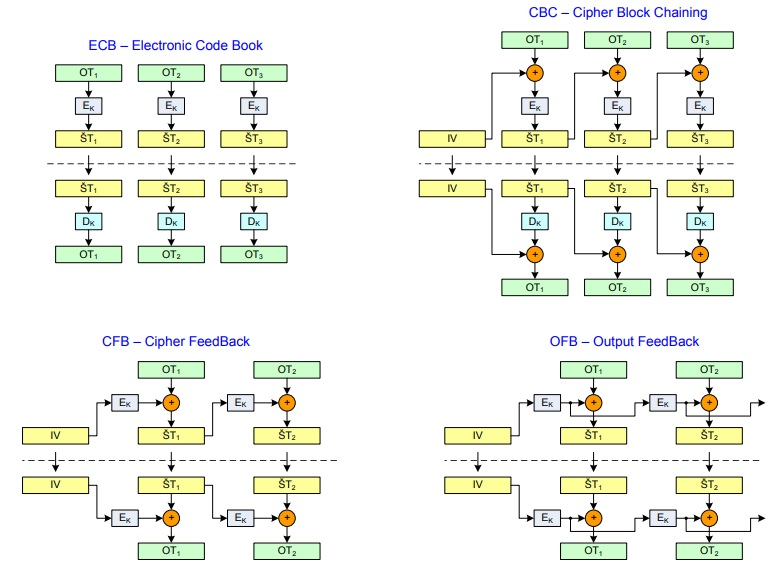
\includegraphics[width=0.9\textwidth]{img/SP-10_0.jpg}
	
	\item CTR (čítačový mód)
	\begin{itemize}
		\item dělá z blokové šifry proudovou (synchronní)
		\item každý blok OT se sečte (xor) s aktuálním heslem z key-streamu, key-stream je nezávislý na OT i ŠT, postupně se generuje použitím čítače (načte se IV, poté se něco přičítá)
		\item 1 bit chyby v ŠT poškodí 1 bit v aktuálním bloku OT
		\item má zaručit maximální periodu hesla
		\item v žádných zprávách šifrovaných tímtéž klíčem nesmí dojít k vygenerování stejného bloku hesla vícekrát --- obsah čítače nesmí být stejný
	\end{itemize}
	\item MAC (message authentication code)
	\begin{itemize}
		\item proudové i blokové šifry zajišťují důvěrnost, ne integritu zpráv
		\item MAC zajišťuje integritu a původ zprávy
		\item použije se jiný klíč než k šifrování
		\item funguje jako CBC s nulovým IV, průběžný ŠT se neodesílá
		\item MAC je tvořen posledním blokem ŠT$_n$
	\end{itemize}
	
	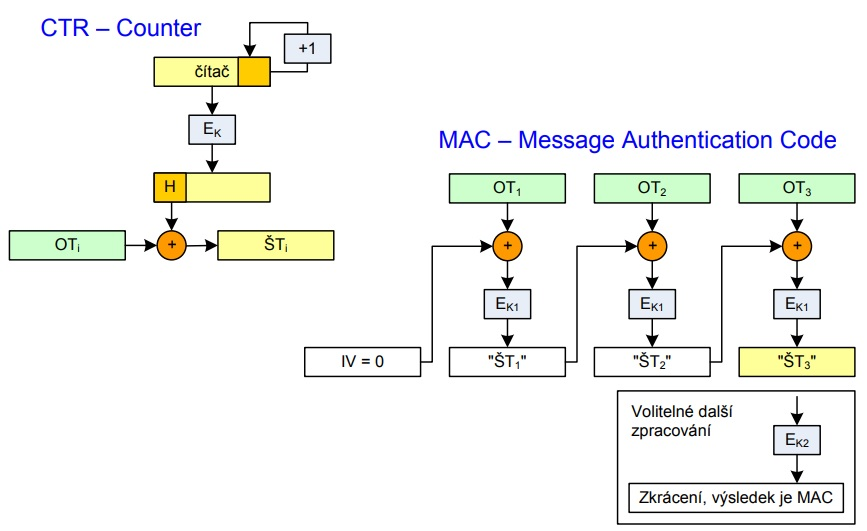
\includegraphics[width=0.9\textwidth]{img/SP-10_1.jpg}
\end{itemize}